\documentclass[12pt]{article}
\usepackage{parskip}
\usepackage[letterpaper, margin=1in]{geometry}
\usepackage{graphicx}
\usepackage{amsmath}
\usepackage{enumitem}
\usepackage{caption}
\usepackage{subcaption}
\usepackage{hyperref}
\graphicspath{{./images/}}
\title{ELECENG 3EJ4 Lab 3}
\author{Raeed Hassan \\ hassam41 \\ McMaster University}
\begin{document}
\maketitle
\pagebreak
\begin{itemize}
    \section*{Part 1}
    \item [\textbf{Q1.}]
    \begin{enumerate}
        \item The relationship between $I_o$ and $I_{REF}$ is dependent on the EBJ area of the two BJTs. As the two BJTs are the same, they have the same EBJ area and the relationship between $I_o$ and $I_{REF}$ can be described as:
        \begin{equation*}
            I_o = I_{REF}
        \end{equation*}
        \item When $I_{REF}$ is 1 mA, $I_o$ is equal to 0.975 mA, or 0.975$I_{REF}$.
        \item The values of $I_o$ at $I_{REF}$ = 0.1 mA and 1 mA are 1.04$I_{REF}$ and 0.975$I_{REF}$. The theoretical prediction and simulated results are similar, as the simulated results show that $I_o \approx I_{REF}$. 
    \end{enumerate}
    \item [\textbf{Q2.}]
    \begin{enumerate}
        \item The input impedance $R_{in}$ is 389.12 $\Omega$. The current gain $A_i$ is 1.042.
        \item The output resistance $R_o$ is 1.58 M$\Omega$.
        \item The linear two-port network for the current mirror is shown in Figure \ref{fig:q2.3}.
        \begin{figure}[!ht]
            \centering
            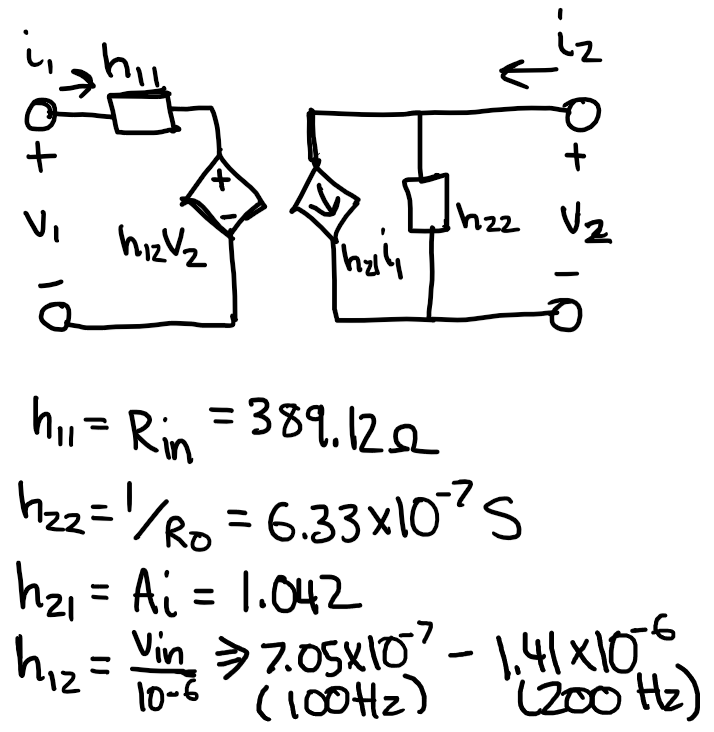
\includegraphics[width=0.65\textwidth]{q2.3}
            \caption{\label{fig:q2.3}Linear two-port network for the current mirror using its $h$-parameters}
        \end{figure}
    \end{enumerate}
    \newpage
    \section*{Part 2}
    \item [\textbf{Q3.}]
    \begin{enumerate}
        \item The voltage gain $A_d$ is 70.07 dB.
        \item The measured voltage gain $A_d$ is 58.1 dB. There was a slight mismatch. The offset voltage applied at $V_2$ was 1 mV.
    \end{enumerate}
    \item [\textbf{Q4.}]
    The upper 3-dB frequency $f_{\text{H}}$ is approximately 11.2 kHz.
    \item [\textbf{Q5.}]
    The upper 3-dB frequency $f_{3\text{dB}}$ of the differential amplifier using resistive loads in Lab 2 was 8.4 MHz, much greater than the differential amplifier with a current mirror in this lab. The differential amplifier with the current mirror load has a smaller $f_{3\text{dB}}$ due to the internal capacitive effects of the BJTs used in the current mirror load.
    \item [\textbf{Q6.}]
    The gain-bandwidth product of the differential amplifier with the current mirror load is 151.1, while the gain-bandwidth product of the differential amplifier with the resistive load is 152.0.
\end{itemize}
\newpage
\section*{Appendix}
\begin{figure}[!ht]
    \centering
    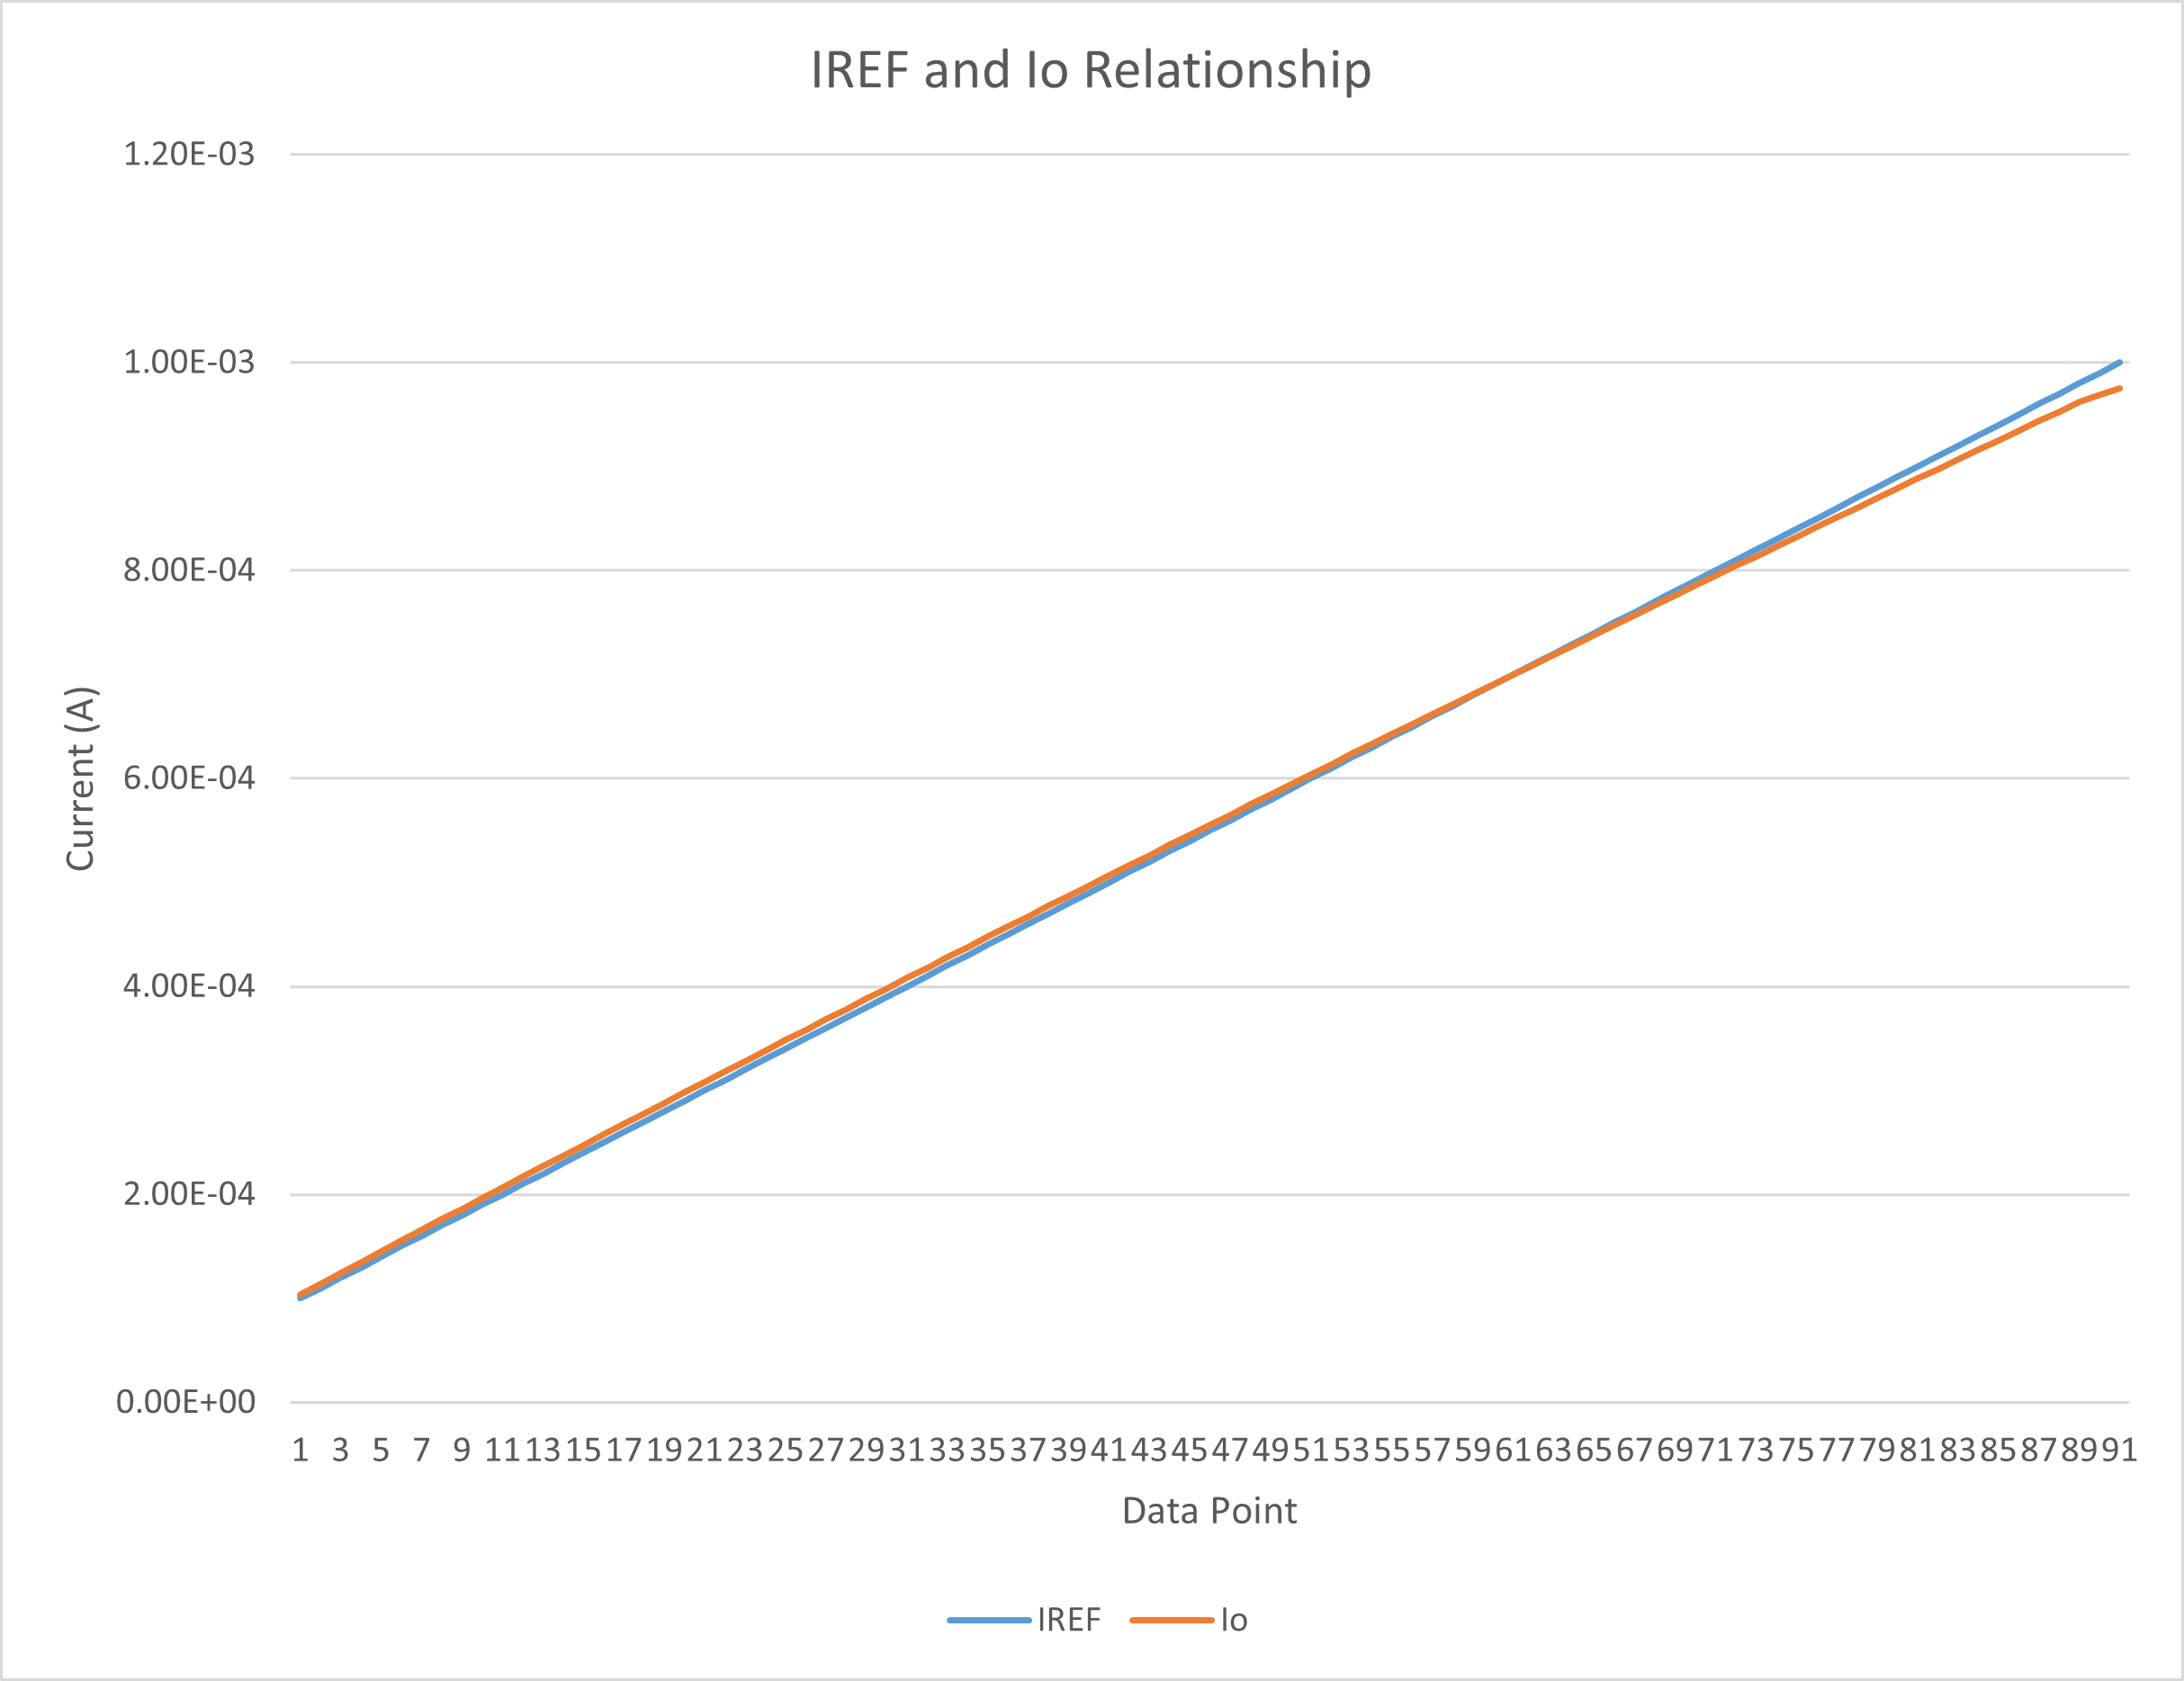
\includegraphics[width=0.7\textwidth]{Step1.2}
    \caption{\label{fig:step1.2}Step 1.2}
\end{figure}
\begin{figure}[!ht]
    \centering
    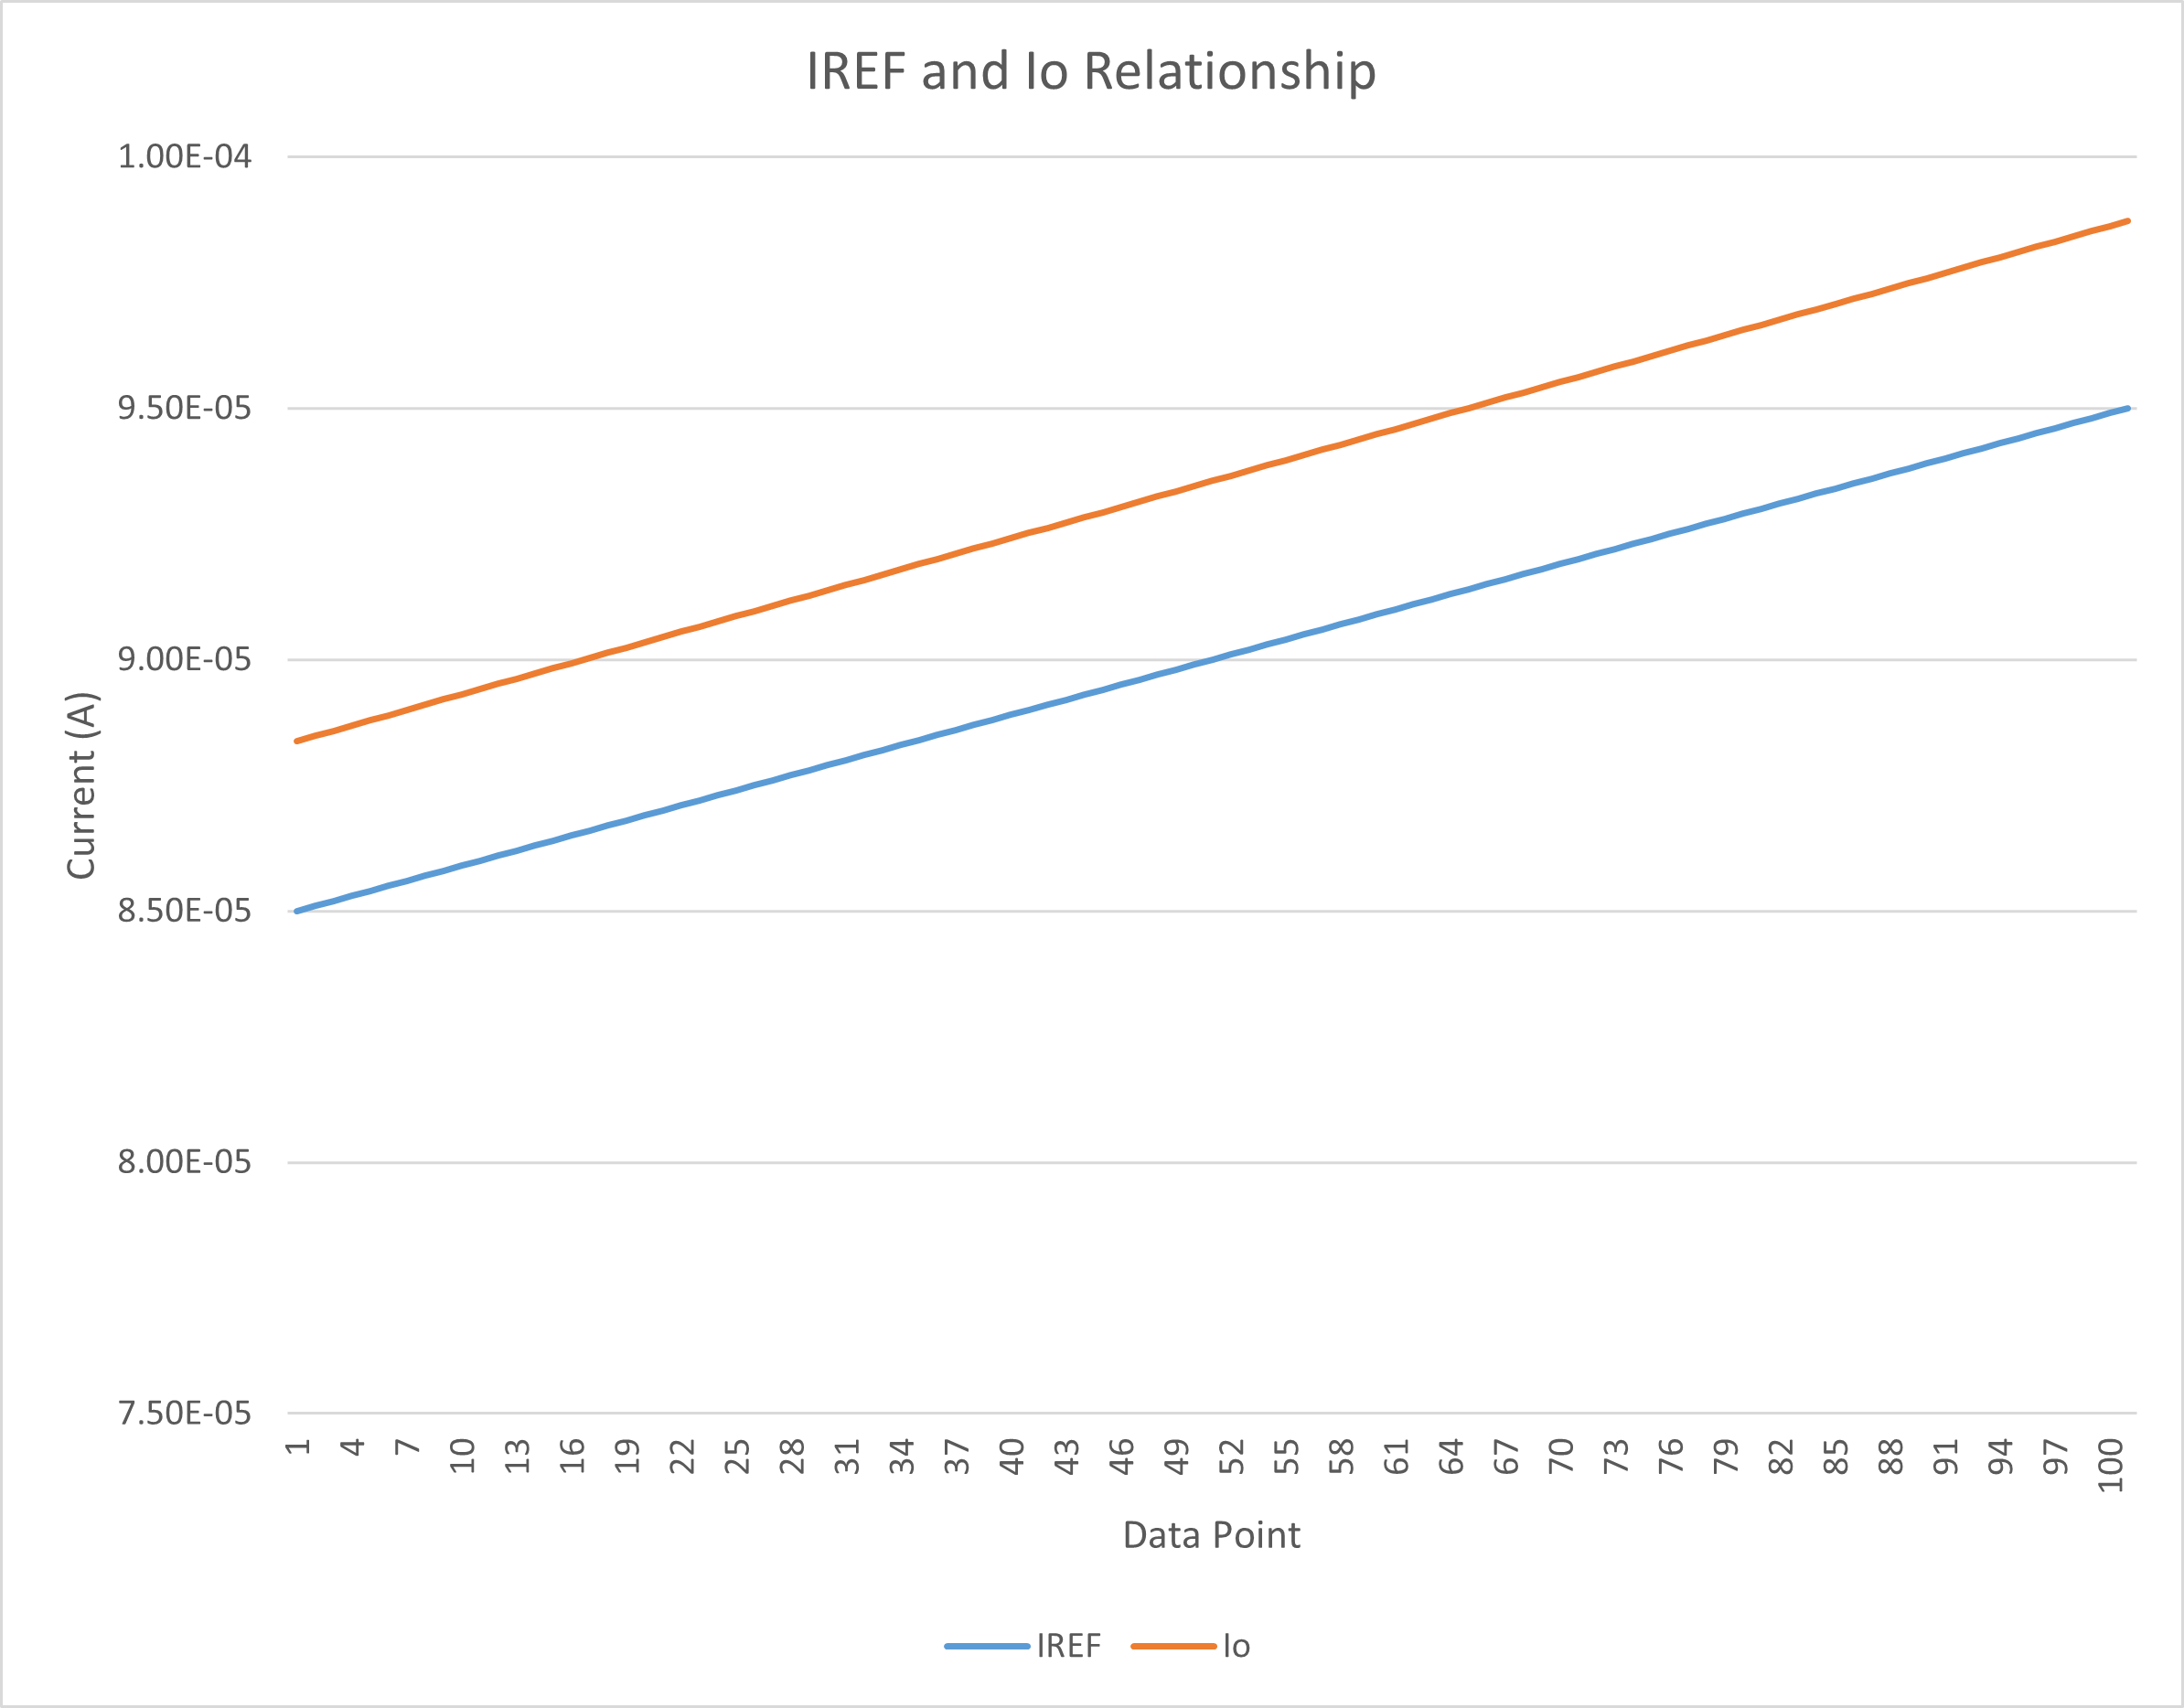
\includegraphics[width=0.7\textwidth]{Step1.3}
    \caption{\label{fig:step1.3}Step 1.3}
\end{figure}
\begin{figure}[!ht]
    \centering
    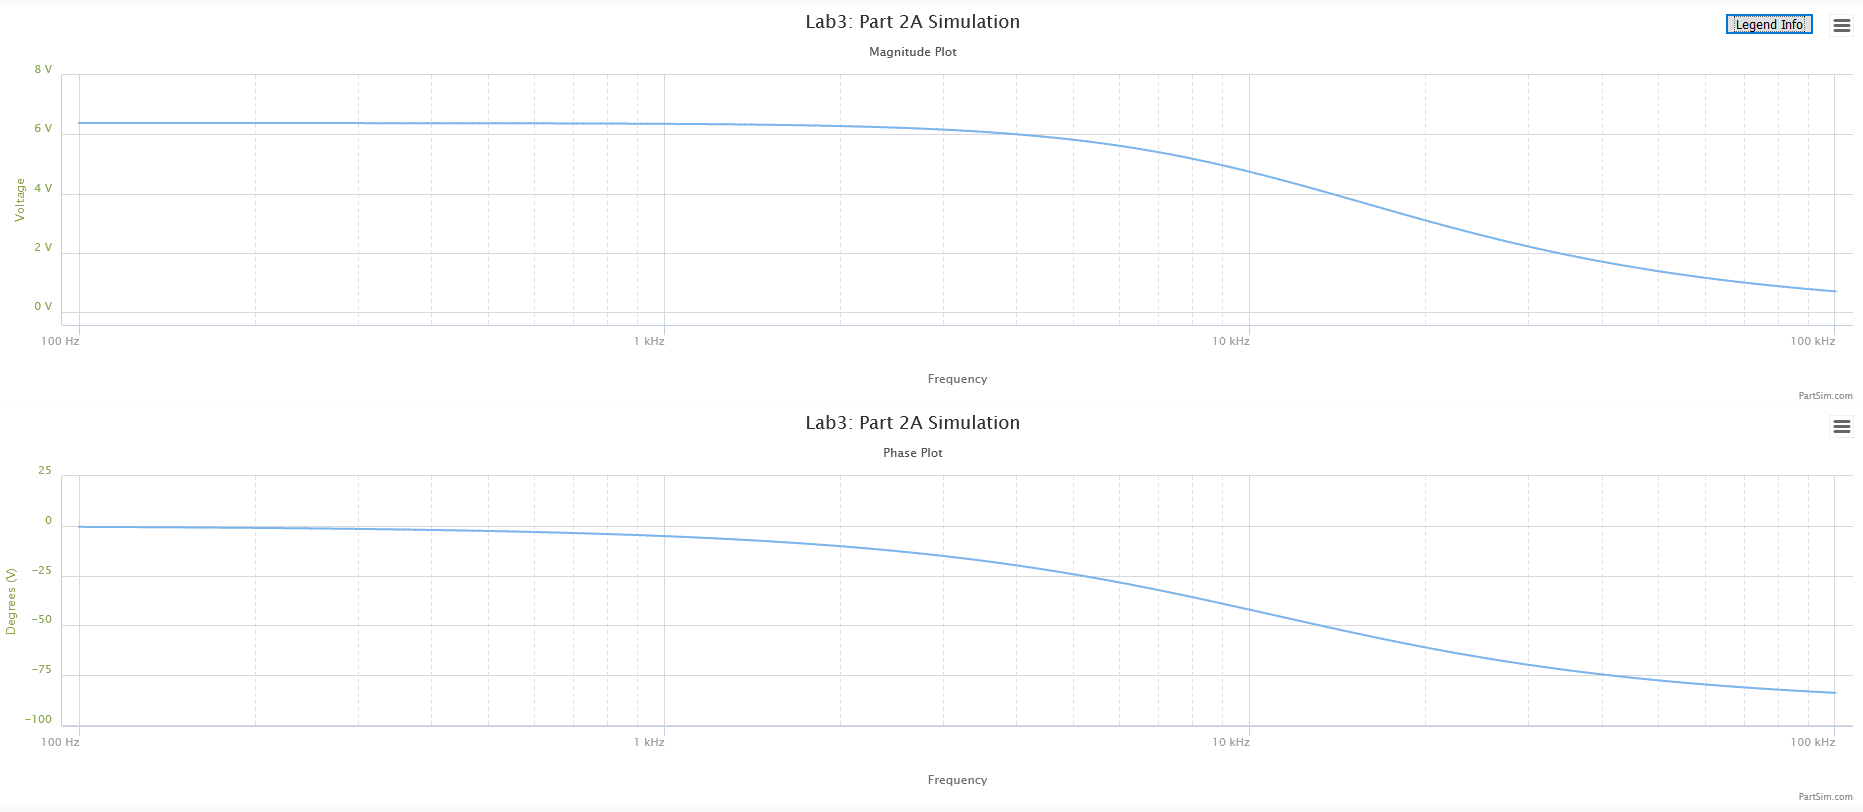
\includegraphics[width=\textwidth]{part2bode}
    \caption{\label{fig:bode}Bode plots for Part 2A}
\end{figure}
\begin{figure}[!ht]
    \centering
    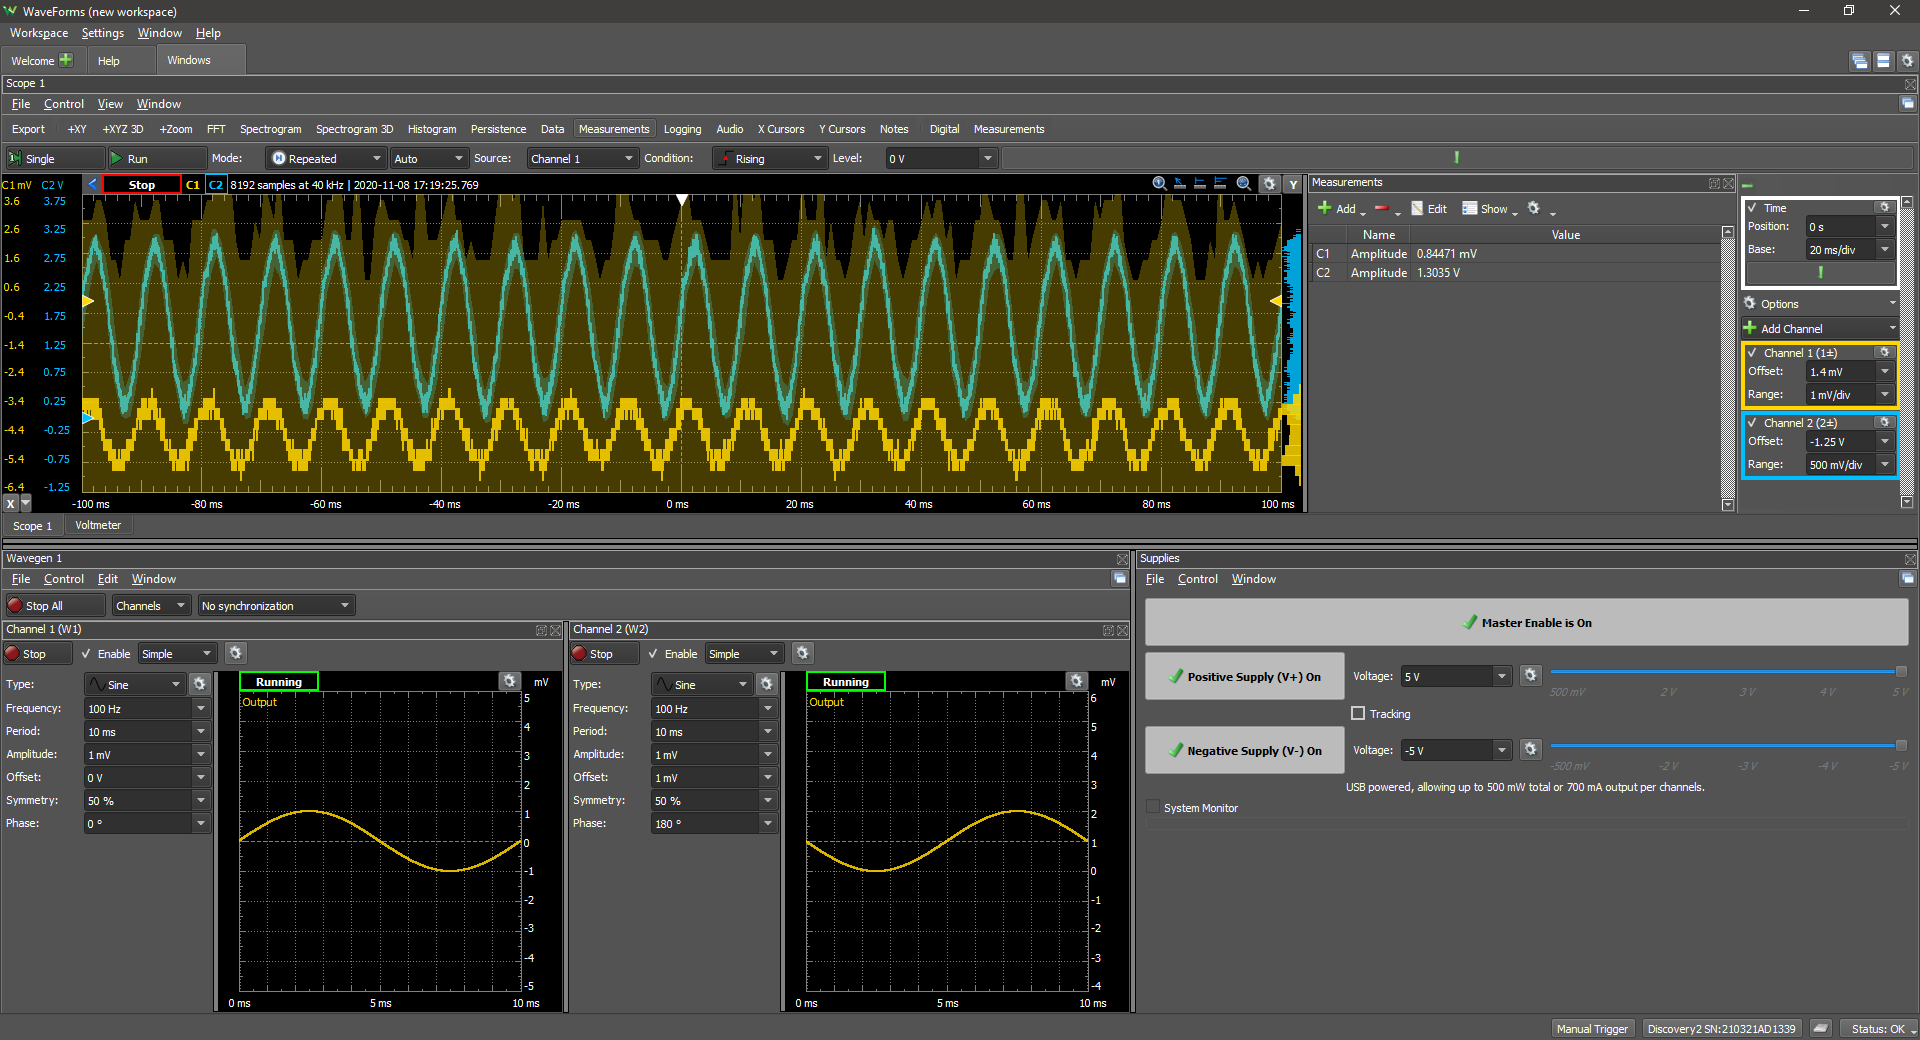
\includegraphics[width=\textwidth]{part2waves}
    \caption{\label{fig:waves}Waveforms Window for Part 2B}
\end{figure}
\begin{figure}[!ht]
    \centering
    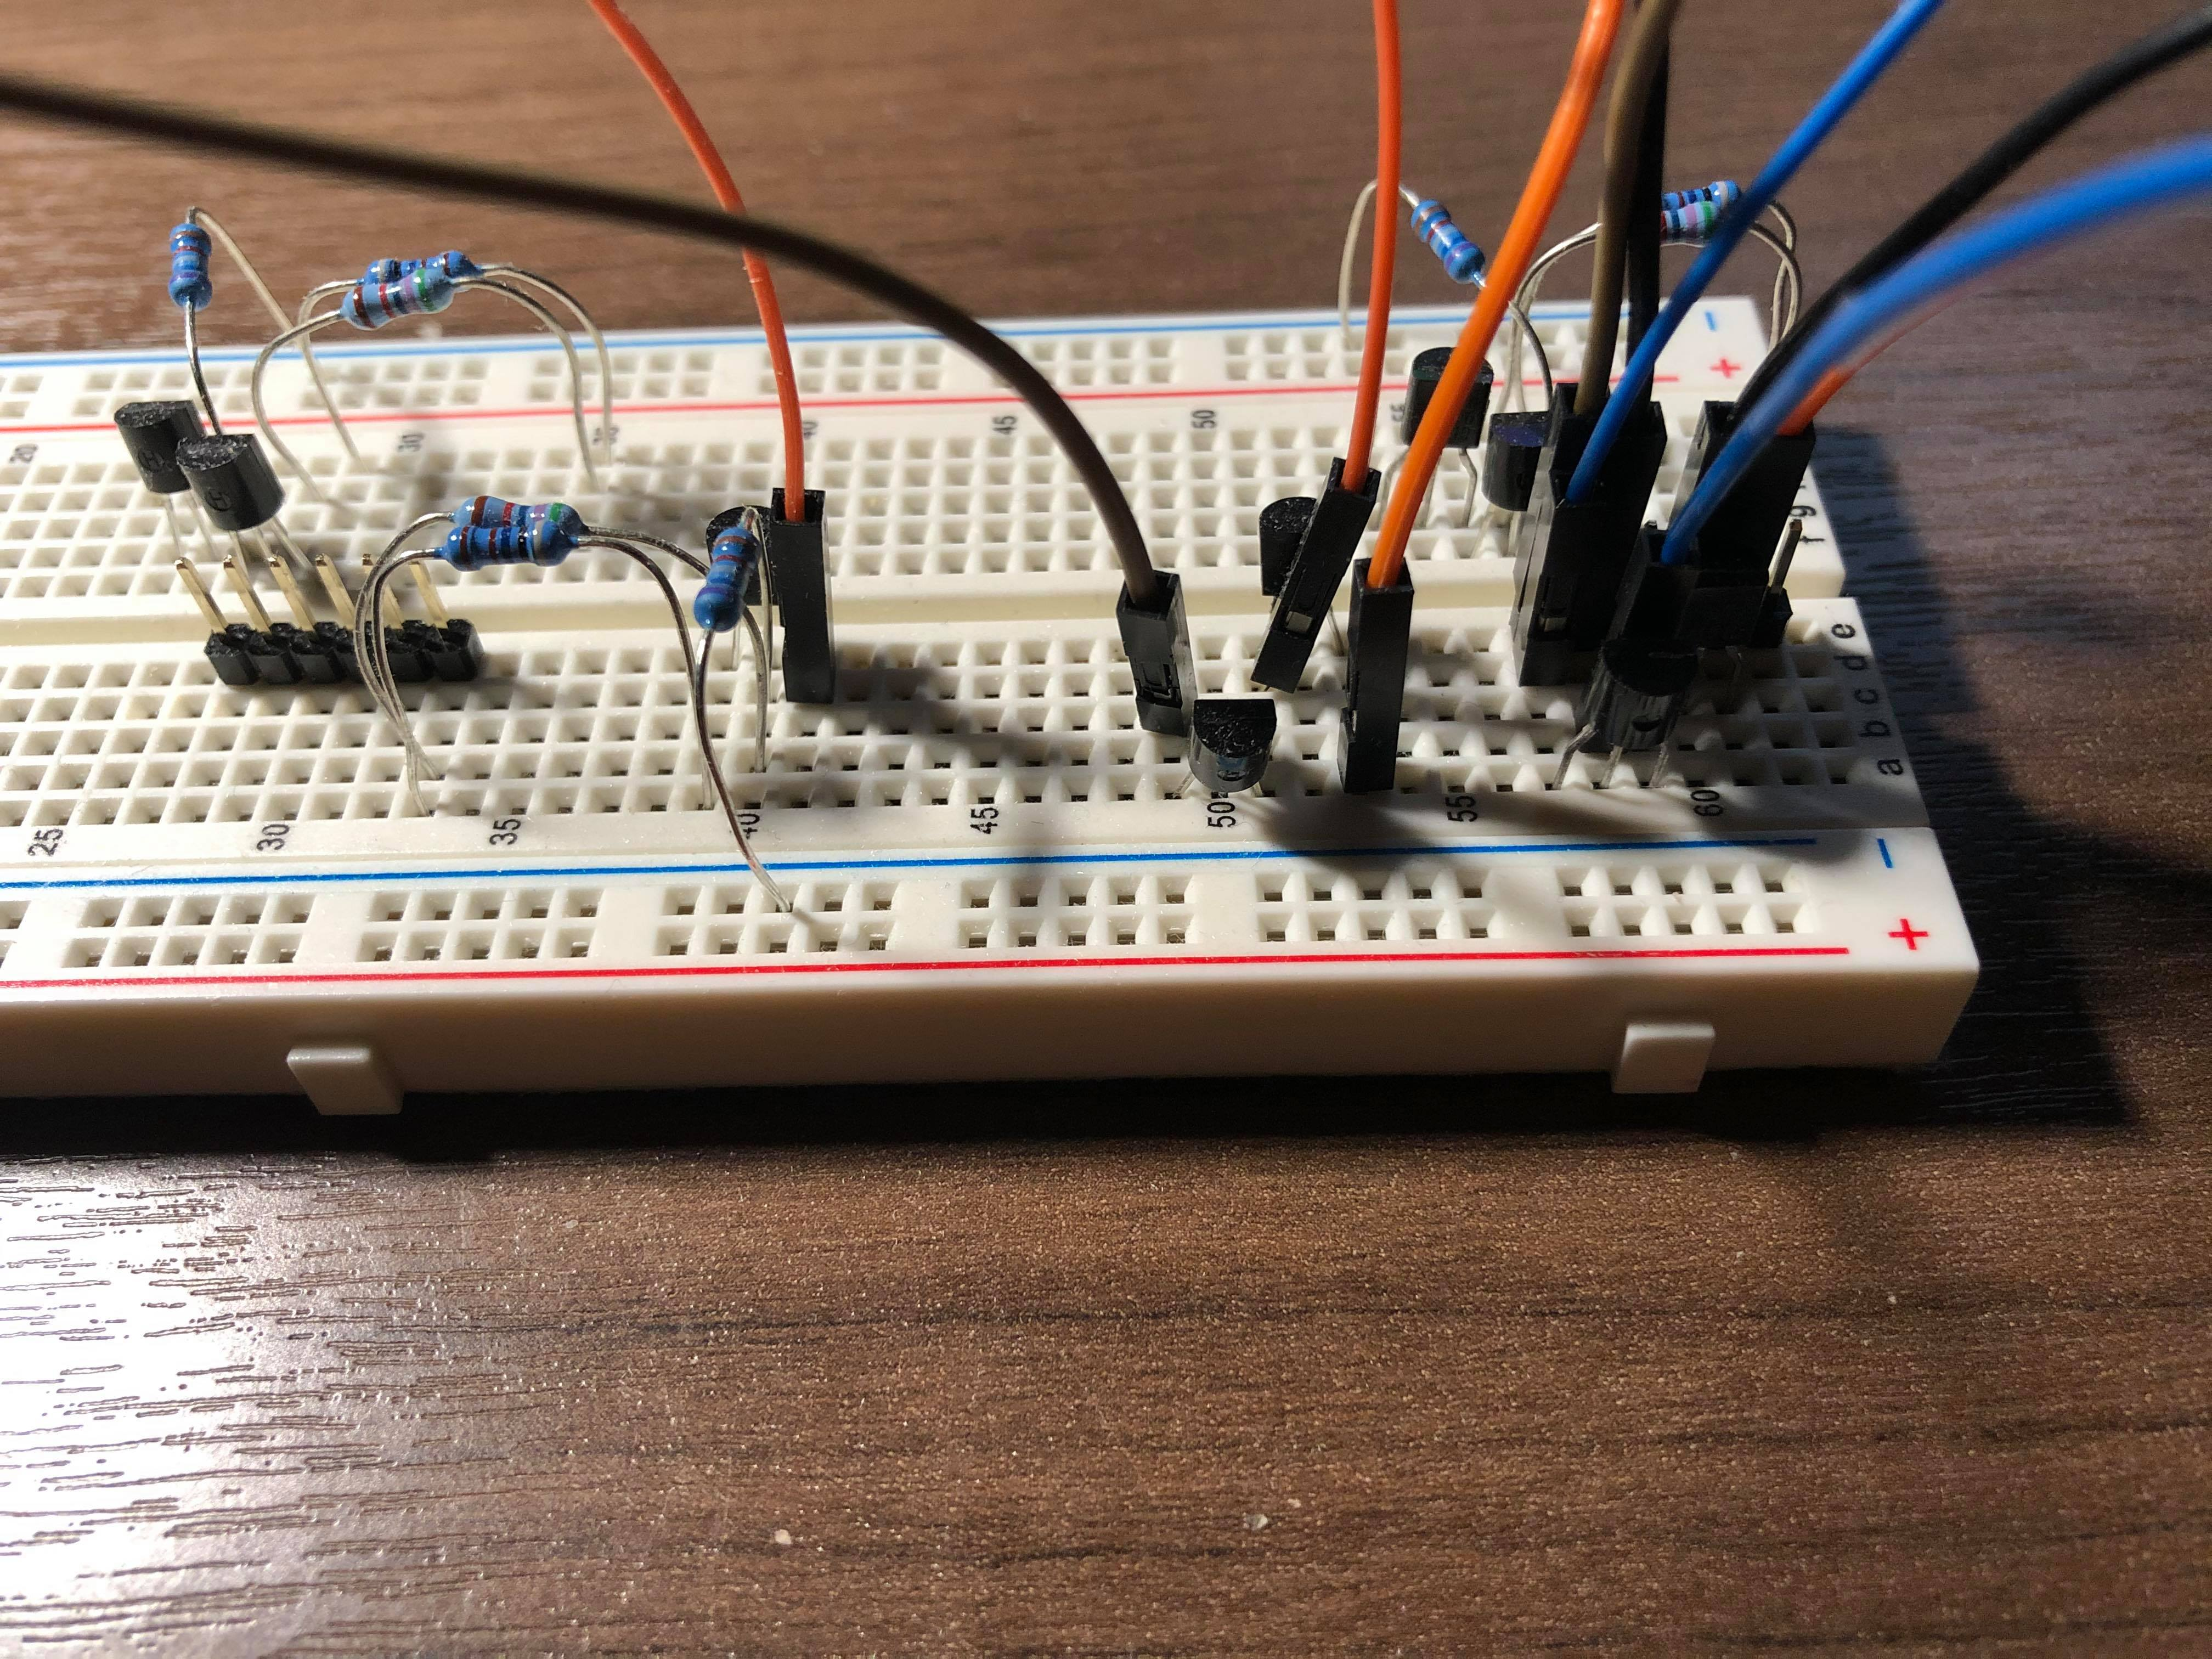
\includegraphics[width=\textwidth]{circuit}
    \caption{\label{fig:circuit}Circuit for Part 2B}
\end{figure}
\end{document}